% Options for packages loaded elsewhere
% Options for packages loaded elsewhere
\PassOptionsToPackage{unicode}{hyperref}
\PassOptionsToPackage{hyphens}{url}
\PassOptionsToPackage{dvipsnames,svgnames,x11names}{xcolor}
%
\documentclass[
  chinese,
]{ctexart}
\usepackage{xcolor}
\usepackage[margin=1in]{geometry}
\usepackage{amsmath,amssymb}
\setcounter{secnumdepth}{-\maxdimen} % remove section numbering
\usepackage{iftex}
\ifPDFTeX
  \usepackage[T1]{fontenc}
  \usepackage[utf8]{inputenc}
  \usepackage{textcomp} % provide euro and other symbols
\else % if luatex or xetex
  \usepackage{unicode-math} % this also loads fontspec
  \defaultfontfeatures{Scale=MatchLowercase}
  \defaultfontfeatures[\rmfamily]{Ligatures=TeX,Scale=1}
\fi
\usepackage{lmodern}
\ifPDFTeX\else
  % xetex/luatex font selection
\fi
% Use upquote if available, for straight quotes in verbatim environments
\IfFileExists{upquote.sty}{\usepackage{upquote}}{}
\IfFileExists{microtype.sty}{% use microtype if available
  \usepackage[]{microtype}
  \UseMicrotypeSet[protrusion]{basicmath} % disable protrusion for tt fonts
}{}
\makeatletter
\@ifundefined{KOMAClassName}{% if non-KOMA class
  \IfFileExists{parskip.sty}{%
    \usepackage{parskip}
  }{% else
    \setlength{\parindent}{0pt}
    \setlength{\parskip}{6pt plus 2pt minus 1pt}}
}{% if KOMA class
  \KOMAoptions{parskip=half}}
\makeatother
% Make \paragraph and \subparagraph free-standing
\makeatletter
\ifx\paragraph\undefined\else
  \let\oldparagraph\paragraph
  \renewcommand{\paragraph}{
    \@ifstar
      \xxxParagraphStar
      \xxxParagraphNoStar
  }
  \newcommand{\xxxParagraphStar}[1]{\oldparagraph*{#1}\mbox{}}
  \newcommand{\xxxParagraphNoStar}[1]{\oldparagraph{#1}\mbox{}}
\fi
\ifx\subparagraph\undefined\else
  \let\oldsubparagraph\subparagraph
  \renewcommand{\subparagraph}{
    \@ifstar
      \xxxSubParagraphStar
      \xxxSubParagraphNoStar
  }
  \newcommand{\xxxSubParagraphStar}[1]{\oldsubparagraph*{#1}\mbox{}}
  \newcommand{\xxxSubParagraphNoStar}[1]{\oldsubparagraph{#1}\mbox{}}
\fi
\makeatother

\usepackage{color}
\usepackage{fancyvrb}
\newcommand{\VerbBar}{|}
\newcommand{\VERB}{\Verb[commandchars=\\\{\}]}
\DefineVerbatimEnvironment{Highlighting}{Verbatim}{commandchars=\\\{\}}
% Add ',fontsize=\small' for more characters per line
\usepackage{framed}
\definecolor{shadecolor}{RGB}{241,243,245}
\newenvironment{Shaded}{\begin{snugshade}}{\end{snugshade}}
\newcommand{\AlertTok}[1]{\textcolor[rgb]{0.68,0.00,0.00}{#1}}
\newcommand{\AnnotationTok}[1]{\textcolor[rgb]{0.37,0.37,0.37}{#1}}
\newcommand{\AttributeTok}[1]{\textcolor[rgb]{0.40,0.45,0.13}{#1}}
\newcommand{\BaseNTok}[1]{\textcolor[rgb]{0.68,0.00,0.00}{#1}}
\newcommand{\BuiltInTok}[1]{\textcolor[rgb]{0.00,0.23,0.31}{#1}}
\newcommand{\CharTok}[1]{\textcolor[rgb]{0.13,0.47,0.30}{#1}}
\newcommand{\CommentTok}[1]{\textcolor[rgb]{0.37,0.37,0.37}{#1}}
\newcommand{\CommentVarTok}[1]{\textcolor[rgb]{0.37,0.37,0.37}{\textit{#1}}}
\newcommand{\ConstantTok}[1]{\textcolor[rgb]{0.56,0.35,0.01}{#1}}
\newcommand{\ControlFlowTok}[1]{\textcolor[rgb]{0.00,0.23,0.31}{\textbf{#1}}}
\newcommand{\DataTypeTok}[1]{\textcolor[rgb]{0.68,0.00,0.00}{#1}}
\newcommand{\DecValTok}[1]{\textcolor[rgb]{0.68,0.00,0.00}{#1}}
\newcommand{\DocumentationTok}[1]{\textcolor[rgb]{0.37,0.37,0.37}{\textit{#1}}}
\newcommand{\ErrorTok}[1]{\textcolor[rgb]{0.68,0.00,0.00}{#1}}
\newcommand{\ExtensionTok}[1]{\textcolor[rgb]{0.00,0.23,0.31}{#1}}
\newcommand{\FloatTok}[1]{\textcolor[rgb]{0.68,0.00,0.00}{#1}}
\newcommand{\FunctionTok}[1]{\textcolor[rgb]{0.28,0.35,0.67}{#1}}
\newcommand{\ImportTok}[1]{\textcolor[rgb]{0.00,0.46,0.62}{#1}}
\newcommand{\InformationTok}[1]{\textcolor[rgb]{0.37,0.37,0.37}{#1}}
\newcommand{\KeywordTok}[1]{\textcolor[rgb]{0.00,0.23,0.31}{\textbf{#1}}}
\newcommand{\NormalTok}[1]{\textcolor[rgb]{0.00,0.23,0.31}{#1}}
\newcommand{\OperatorTok}[1]{\textcolor[rgb]{0.37,0.37,0.37}{#1}}
\newcommand{\OtherTok}[1]{\textcolor[rgb]{0.00,0.23,0.31}{#1}}
\newcommand{\PreprocessorTok}[1]{\textcolor[rgb]{0.68,0.00,0.00}{#1}}
\newcommand{\RegionMarkerTok}[1]{\textcolor[rgb]{0.00,0.23,0.31}{#1}}
\newcommand{\SpecialCharTok}[1]{\textcolor[rgb]{0.37,0.37,0.37}{#1}}
\newcommand{\SpecialStringTok}[1]{\textcolor[rgb]{0.13,0.47,0.30}{#1}}
\newcommand{\StringTok}[1]{\textcolor[rgb]{0.13,0.47,0.30}{#1}}
\newcommand{\VariableTok}[1]{\textcolor[rgb]{0.07,0.07,0.07}{#1}}
\newcommand{\VerbatimStringTok}[1]{\textcolor[rgb]{0.13,0.47,0.30}{#1}}
\newcommand{\WarningTok}[1]{\textcolor[rgb]{0.37,0.37,0.37}{\textit{#1}}}

\usepackage{longtable,booktabs,array}
\newcounter{none} % for unnumbered tables
\usepackage{calc} % for calculating minipage widths
% Correct order of tables after \paragraph or \subparagraph
\usepackage{etoolbox}
\makeatletter
\patchcmd\longtable{\par}{\if@noskipsec\mbox{}\fi\par}{}{}
\makeatother
% Allow footnotes in longtable head/foot
\IfFileExists{footnotehyper.sty}{\usepackage{footnotehyper}}{\usepackage{footnote}}
\makesavenoteenv{longtable}
\usepackage{graphicx}
\makeatletter
\newsavebox\pandoc@box
\newcommand*\pandocbounded[1]{% scales image to fit in text height/width
  \sbox\pandoc@box{#1}%
  \Gscale@div\@tempa{\textheight}{\dimexpr\ht\pandoc@box+\dp\pandoc@box\relax}%
  \Gscale@div\@tempb{\linewidth}{\wd\pandoc@box}%
  \ifdim\@tempb\p@<\@tempa\p@\let\@tempa\@tempb\fi% select the smaller of both
  \ifdim\@tempa\p@<\p@\scalebox{\@tempa}{\usebox\pandoc@box}%
  \else\usebox{\pandoc@box}%
  \fi%
}
% Set default figure placement to htbp
\def\fps@figure{htbp}
\makeatother



\ifLuaTeX
\usepackage[bidi=basic,shorthands=off,provide=*]{babel}
\else
\usepackage[bidi=default,shorthands=off,provide=*]{babel}
\fi
\ifLuaTeX
  \usepackage{selnolig} % disable illegal ligatures
\fi


\setlength{\emergencystretch}{3em} % prevent overfull lines

\providecommand{\tightlist}{%
  \setlength{\itemsep}{0pt}\setlength{\parskip}{0pt}}



 


\usepackage{fvextra}
\DefineVerbatimEnvironment{Highlighting}{Verbatim}{breaklines,breakanywhere,commandchars=\\\{\}}
\usepackage{changepage}
\usepackage{xcolor}
\usepackage{dirtree}
\definecolor{TreeNoteColor}{RGB}{120,98,78}
\renewcommand*\DTstyle{\ttfamily\small}
\makeatletter
\@ifpackageloaded{caption}{}{\usepackage{caption}}
\AtBeginDocument{%
\ifdefined\contentsname
  \renewcommand*\contentsname{目录}
\else
  \newcommand\contentsname{目录}
\fi
\ifdefined\listfigurename
  \renewcommand*\listfigurename{图索引}
\else
  \newcommand\listfigurename{图索引}
\fi
\ifdefined\listtablename
  \renewcommand*\listtablename{表索引}
\else
  \newcommand\listtablename{表索引}
\fi
\ifdefined\figurename
  \renewcommand*\figurename{图}
\else
  \newcommand\figurename{图}
\fi
\ifdefined\tablename
  \renewcommand*\tablename{表}
\else
  \newcommand\tablename{表}
\fi
}
\@ifpackageloaded{float}{}{\usepackage{float}}
\floatstyle{ruled}
\@ifundefined{c@chapter}{\newfloat{codelisting}{h}{lop}}{\newfloat{codelisting}{h}{lop}[chapter]}
\floatname{codelisting}{列表}
\newcommand*\listoflistings{\listof{codelisting}{列表索引}}
\makeatother
\makeatletter
\makeatother
\makeatletter
\@ifpackageloaded{caption}{}{\usepackage{caption}}
\@ifpackageloaded{subcaption}{}{\usepackage{subcaption}}
\makeatother
\usepackage{bookmark}
\IfFileExists{xurl.sty}{\usepackage{xurl}}{} % add URL line breaks if available
\urlstyle{same}
% fallback for those not using the hyperref driver hyperxmp:
\makeatletter
\@ifundefined{xmpquote}{\newcommand{\xmpquote}[1]{#1}}{}
\makeatother
\hypersetup{
  pdftitle={第8讲 端到端策略导论：从 Pipeline 到 Policy},
  pdflang={zh-CN},
  colorlinks=true,
  linkcolor={blue},
  filecolor={Maroon},
  citecolor={Blue},
  urlcolor={Blue},
  pdfcreator={LaTeX via pandoc}}


\title{第8讲 端到端策略导论：从 Pipeline 到 Policy}
\author{}
\date{}
\begin{document}
\maketitle

\renewcommand*\contentsname{目录}
{
\setcounter{tocdepth}{3}
\tableofcontents
}

\section{1 两种机器人：手写 pipeline 还是端到端
policy}\label{ux4e24ux79cdux673aux5668ux4ebaux624bux5199-pipeline-ux8fd8ux662fux7aefux5230ux7aef-policy}

第7讲我们已经让机械臂把红色方块从 A 区搬到了 B
区、把竖直的瓶子放进了收纳盒。用的办法是一条\textbf{人写的流水线}：先估出物体位姿，再算出预抓取、抓取、抬升、放置、退出这五个关键位姿，串成一个状态机，最后逐段执行、逐段校验，失败了还要按阶段回溯排查。它能跑通------代价是每一环的规则都得我们自己写出来。

这一讲把同一件事换一种做法：不再写规则，而是直接用一个神经网络，从相机画面映射到机器人指令。两种做法摆在一起对比，会引出第8到13讲共同的主角------\textbf{策略（policy）}。

\subsection{1.1
传统机器人怎么干活：一条手写的流水线}\label{ux4f20ux7edfux673aux5668ux4ebaux600eux4e48ux5e72ux6d3bux4e00ux6761ux624bux5199ux7684ux6d41ux6c34ux7ebf}

传统做法会把''怎么动''\textbf{显式地}用人写的模型一步步算出来：先感知与建图，再规划一条轨迹，最后交给控制器执行。规划这一步常用两类算法------\textbf{RRT}（快速扩展随机树，Rapidly-exploring
Random
Tree）在自由空间里随机撒点、连成一条不碰东西的路径；\textbf{MPC}（模型预测控制，Model
Predictive
Control）则用动力学模型往前推演几步，再决定当下这一步怎么动。每一环都是人设计出来的。

把''生成机器人运动''的方法摊开看，大致分成两支{[}1{]}：左边是这种\textbf{显式建模}（explicit
modeling：运动学、规划、控制），右边是这一讲要讲的\textbf{隐式建模}（implicit
modeling：从示教中学习、强化学习）：

\begin{figure}[H]

{\centering 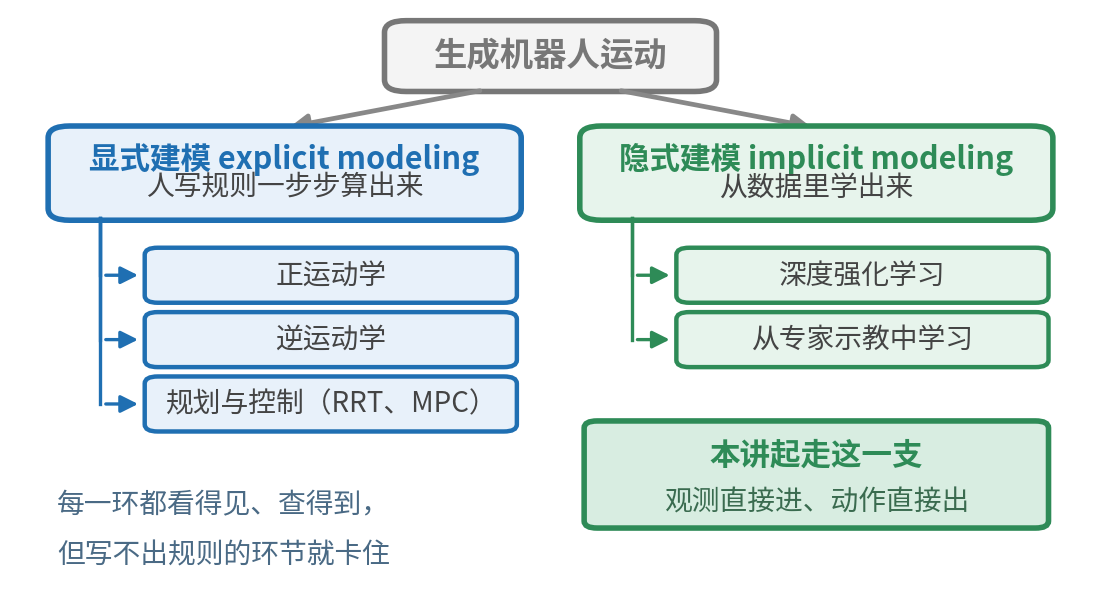
\includegraphics[width=1\linewidth,height=\textheight,keepaspectratio]{../../assets/figures/lecture08/ref/fig08-1-motion-taxonomy.png}

}

\caption{生成机器人运动分成两支：左支显式建模，下挂正运动学、逆运动学、规划与控制（RRT、MPC）三类人写规则的方法；右支隐式建模，下挂深度强化学习与从专家示教中学习。右支底下那个加粗的绿框标出了本讲的落点------观测直接进、动作直接出（本书自绘）}

\end{figure}%

图上要看的不只是''分成两支''，还有那个绿色落点：这一讲以及往后的第9--13讲，全都站在右边这一支上。左支的好处写在它下面------每一步都看得见、查得到，哪里出错就去修哪一段，可解释、可调试。

\subsection{1.2
流水线的死穴：有些环节根本写不出规则}\label{ux6d41ux6c34ux7ebfux7684ux6b7bux7a74ux6709ux4e9bux73afux8282ux6839ux672cux5199ux4e0dux51faux89c4ux5219}

问题在于，\textbf{有些环节是写不出规则的}。

抓一块软布、把线穿进针眼、拧一个滑手的瓶盖------这些任务里物体会形变、会打滑，接触力瞬息万变，你很难用解析模型把''此刻该怎么动''描述清楚。再加上真实世界的长尾层出不穷：换个光照、换个没见过的杯子，手写的感知和规划就要重新调一遍。

流水线不是不好，而是它把''难以言说''的技能硬拆成可编程的步骤，恰恰在最难的那几环上卡住了。

\subsection{1.3
换个思路：让一个网络从观测直接到动作}\label{ux6362ux4e2aux601dux8defux8ba9ux4e00ux4e2aux7f51ux7edcux4eceux89c2ux6d4bux76f4ux63a5ux5230ux52a8ux4f5c}

端到端（end-to-end）策略给出的答案是：\textbf{不再把任务拆成感知---规划---控制三段分别设计，而是用一个神经网络，从图像与状态直接预测任务级的动作表示}，靠联合训练省掉人工写死的中间接口。相机像素进去，动作出来------但要注意这个''动作''通常还不是电机级命令：它更常是关节目标、末端增量或一段动作块，后面仍要经过坐标变换、控制器和安全约束才真正落到电机上。

\begin{quote}
备注：端到端\textbf{不是}要取代一切。端到端强调的是目标函数可以联合优化，不是输出必须直达电机。正逆运动学、安全限位、底层伺服这些有成熟解析解的部分仍然保留；端到端替代的，是那几个''写不出规则''的环节。
\end{quote}

最早把这件事讲清楚的两个工作，一个在自动驾驶、一个在机械臂。NVIDIA 的
\textbf{DAVE-2}{[}2{]}
让摄像头画面直接进一个卷积网络、输出方向盘转角，中间不再有''车道线检测→路径规划→转向控制''的人工流水线。这个名字来自
2016 年那篇原始论文；同一组人在 2017 年的后续工作里把它改称
\textbf{PilotNet}{[}3{]}，今天多数人是用后一个名字记住它的：

\begin{figure}[H]

{\centering \pandocbounded{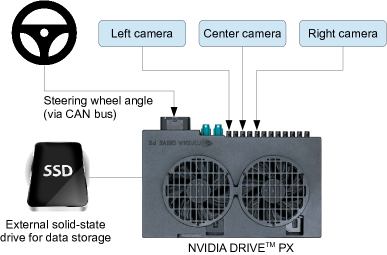
\includegraphics[keepaspectratio]{../../assets/figures/lecture08/ref/813_pilotnet-end2end_arxiv-1604.07316.png}}

}

\caption{NVIDIA DAVE-2（后称
PilotNet）：摄像头图像经一个卷积网络直接输出方向盘转角，端到端反向传播训练}

\end{figure}%

Levine
等人{[}4{]}在机械臂上做了同样的事，用一个网络把图像直接映射到电机扭矩。他们问的是同一个问题：把感知和控制\textbf{联合}训练，会不会比分开设计更好？在他们那组视觉运动控制任务上，答案是肯定的------联合训练的策略优于所比较的分阶段基线。这是那批任务、那批数据、那组基线下的结果，不等于所有任务都该取消模块化设计。

\begin{figure}[H]

{\centering \pandocbounded{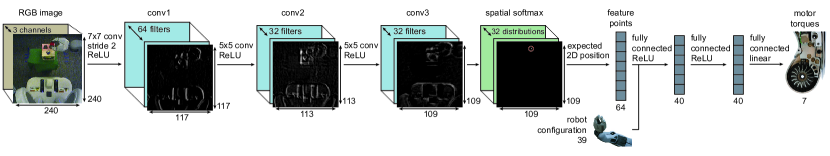
\includegraphics[keepaspectratio]{../../assets/figures/lecture08/ref/813_levine-visuomotor-arch_arxiv-1504.00702.png}}

}

\caption{Levine 视觉运动策略：RGB
图像经卷积与空间特征点提取，直接映射到电机扭矩}

\end{figure}%

把这两件事抽象出来------``那个直接吃观测、吐动作的网络''------就是这一讲真正的主角。

\section{2 什么是 policy}\label{ux4ec0ux4e48ux662f-policy}

\subsection{2.1
一句话定义：从观测到动作的映射}\label{ux4e00ux53e5ux8bddux5b9aux4e49ux4eceux89c2ux6d4bux5230ux52a8ux4f5cux7684ux6620ux5c04}

\begin{quote}
策略（policy）就是一个从\textbf{观测}到\textbf{动作}的函数：你给它当前看到的东西，它告诉你下一步该怎么动。
\end{quote}

放进机器人和环境的互动里看最清楚：\textbf{智能体}（agent，在这里就是机器人）从环境收到观测，输出一个动作作用回环境，环境再给出新的观测------如此往复。这张经典的''智能体---环境''回路就是策略工作的舞台：

\begin{figure}[H]

{\centering 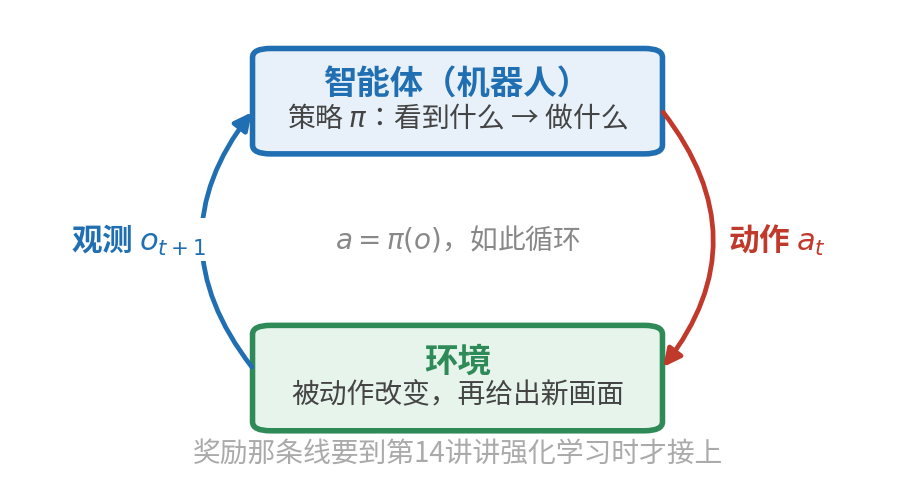
\includegraphics[width=1\linewidth,height=\textheight,keepaspectratio]{../../assets/figures/lecture08/ref/fig08-2-agent-env-loop.png}

}

\caption{智能体与环境只有两条边的闭环：智能体（策略
\(\pi\)）看到观测就给出动作
\(a_t\)，动作作用到环境上，环境被改变后返回新的观测
\(o_{t+1}\)，如此循环（本书自绘）}

\end{figure}%

这张图上只有两条边------动作出去、观测回来，这一讲要的正是这两条。图下那行灰字提醒的是：强化学习那套习惯记号里还有第三条边（奖励
\(r_{t+1}\)），第14讲会把它接上，本讲先不碰。写成符号是
\(a = \pi(o)\)；更一般地写成一个分布
\(\pi(a \mid o)\)------同一个观测下，合理的动作往往不止一个。这件事会成为第10讲
1.4 节的核心出发点。

\begin{center}
\begin{tabular}{@{}>{\raggedright\arraybackslash}p{\dimexpr 0.0879\linewidth - 2\tabcolsep\relax} >{\raggedright\arraybackslash}p{\dimexpr 0.3994\linewidth - 2\tabcolsep\relax} >{\raggedright\arraybackslash}p{\dimexpr 0.5127\linewidth - 2\tabcolsep\relax}@{}}
\toprule\noalign{}
符号 & 含义 & 典型例子 \\
\midrule\noalign{}
\(o\) & observation，观测 & 相机图像、机器人关节角 \\
\(a\) & action，动作 & 各关节目标角度、末端位姿、电机扭矩 \\
\(\pi\) & policy，策略（要学的网络） & 一个卷积 + 全连接网络 \\
\bottomrule\noalign{}
\end{tabular}
\end{center}

\subsection{2.2
观测里有什么、动作又是什么}\label{ux89c2ux6d4bux91ccux6709ux4ec0ux4e48ux52a8ux4f5cux53c8ux662fux4ec0ux4e48}

观测和动作具体长什么样？看一段真实遥操作数据最直观：每一帧的\textbf{观测}
\(o_t\) 由机器人本体状态（关节角
\(q_t\)，那串数字）加上相机图像组成，对应的\textbf{动作} \(a_t\)
是人类专家此刻通过主臂给出的目标关节角------策略要学的，就是''给定上面的观测、回归出下面的动作''：

\begin{figure}[H]

{\centering \pandocbounded{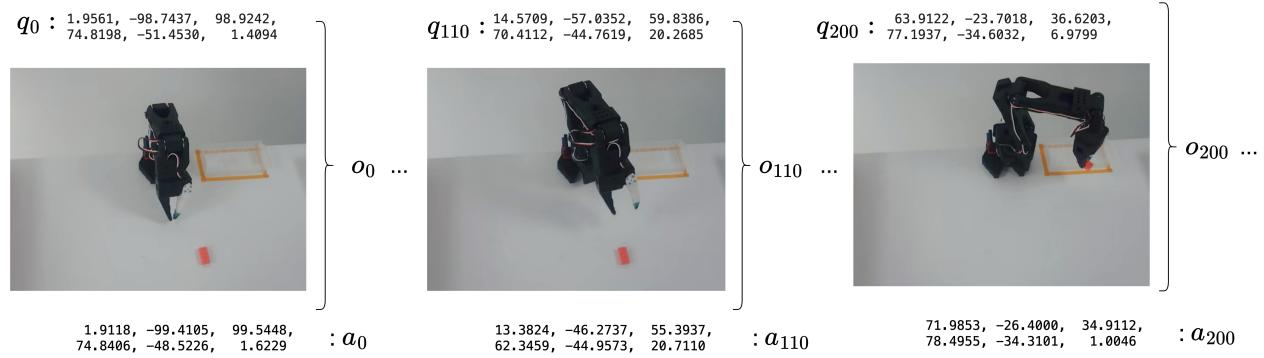
\includegraphics[keepaspectratio]{../../assets/figures/lecture08/ref/822_observation-action-pairs.jpg}}

}

\caption{一段遥操作轨迹里的观测---动作配对：每帧由本体状态加相机图像构成观测，对应人类专家给出的目标关节角作为动作}

\end{figure}%

由此能看清观测和动作各有哪些常见形态：

\textbf{观测 \(o\)
可以是}：本体状态（关节角、末端位置，维度低、信息直接）、图像（信息丰富但要网络自己提取）、语言指令（让同一个策略能做不同任务），以及它们的组合与一小段历史（不只看当前一帧）。

\textbf{动作 \(a\)
的几个关键选择}：在关节空间还是末端空间表达；给\textbf{绝对}目标还是\textbf{相对}增量；一次只预测单步，还是预测未来一小段动作块（action
chunk）。

\begin{quote}
备注：观测和动作的''口径''是策略的接口约定。同一个任务换一种动作表示（比如关节角换成末端位姿、绝对换成相对），对网络来说就是另一个学习问题------后面几讲的很多设计差异，以及第
3 节部署翻车的坑，都出在这里。
\end{quote}

\subsection{2.3 策略的谱系：从只看状态到看懂语言的
VLA}\label{ux7b56ux7565ux7684ux8c31ux7cfbux4eceux53eaux770bux72b6ux6001ux5230ux770bux61c2ux8bedux8a00ux7684-vla}

把''观测里加不加图像、加不加语言''当坐标，策略就排成一条谱系。

最左端是\textbf{状态策略}（state
policy）：观测里只有关节角、末端位置这类本体数字，没有图像。往右一步，观测里加进相机画面，就是\textbf{视觉运动策略}（visuomotor
policy）------第10讲要动手训的 ACT（动作分块 Transformer，Action
Chunking with Transformers）和 Diffusion
Policy（用扩散模型生成动作）都属于这一档。再往右，观测里加进一句自然语言指令，同一个网络就能按''把碗放到盘子上''还是''把杯子推到左边''做不同的事，这类叫\textbf{语言条件策略}（language-conditioned
policy），Google 的 RT-1{[}5{]}
是代表作。最右端把视觉、语言、动作三件事统一进一个大模型，就是\textbf{视觉-语言-动作模型}（Vision-Language-Action，VLA）{[}6{]}，本讲实验要用的
\(\pi_0\) 就是其中一个。

越往右，策略''看懂''的东西越多、能听的指令越泛。把这条谱系画成一条轴：

\begin{figure}[H]

{\centering 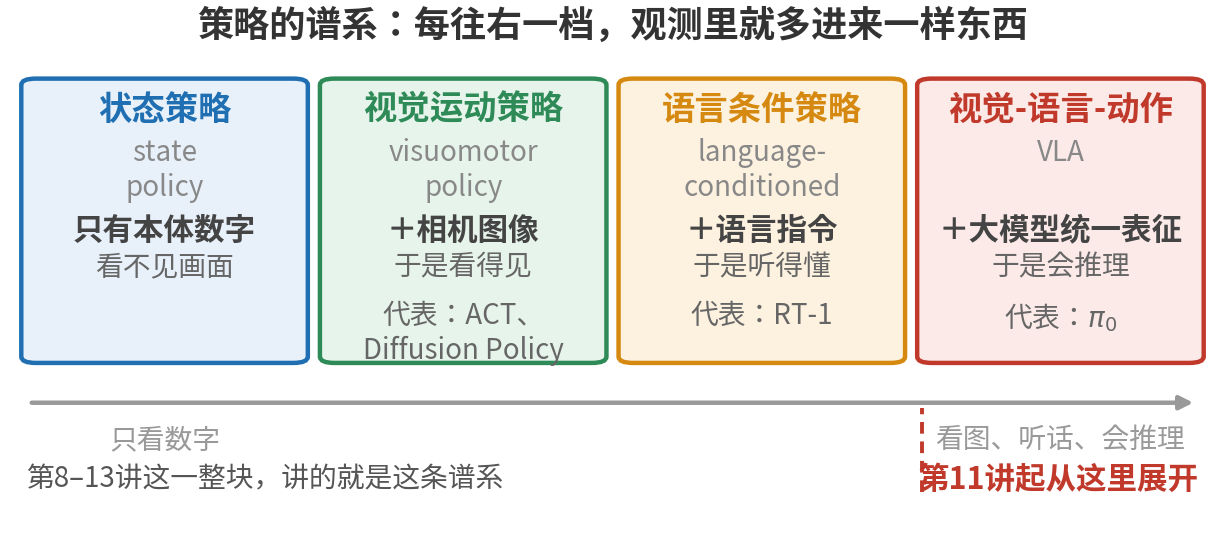
\includegraphics[width=1\linewidth,height=\textheight,keepaspectratio]{../../assets/figures/lecture08/ref/fig08-2-policy-spectrum.png}

}

\caption{策略谱系的四档，从左到右依次是状态策略（state
policy）、视觉运动策略（visuomotor
policy）、语言条件策略（language-conditioned）与视觉-语言-动作模型（VLA）。每一格中间那行加粗字是\textbf{这一档的观测里比左邻多进来的东西}------只有本体数字
/ ＋相机图像 / ＋语言指令 /
＋大模型统一表征，下面一行是它换来的能力与代表方法。最右端那条红色虚线标出第11讲起展开的落点（本书自绘）}

\end{figure}%

图要读的是那一列加粗的''＋``号：四档之间不是四种并列的方法，而是\textbf{同一个
\(\pi(a\mid o)\)
一路往观测里加东西}------先加画面、再加语言、最后加进一个能把两者一起理解的大模型。观测里多进来一样，能听懂的指令就宽一层，这也是为什么最右端的
VLA
能对''把碗放到盘子上''和''把杯子推到左边''做出不同的事。这条谱系正好是本课程''端到端策略''这一大块（第8--13讲）的地图，最右端的
VLA 会从第11讲起展开。

\subsection{2.4 本节小结}\label{ux672cux8282ux5c0fux7ed3}

策略就是''观测→动作''的那个函数，写作
\(\pi(a\mid o)\)。它的两个接口------观测里放什么、动作怎么表达------决定了它是一个只看状态的状态策略，还是一个能听语言的
VLA，也决定了它好不好训、好不好部署。下一节就来看，当我们真把一个策略学出来、搬上机器人时，会在哪些地方栽跟头。

\section{3 从训练到部署：为什么 loss
低了还会失败}\label{ux4eceux8badux7ec3ux5230ux90e8ux7f72ux4e3aux4ec0ux4e48-loss-ux4f4eux4e86ux8fd8ux4f1aux5931ux8d25}

策略是学出来的。但''学得好''和''用得好''之间，隔着几道部署时才会暴露的坎。这一节不讲新算法，讲\textbf{数据的变换}：示教数据在进网络之前，要先统一动作口径、再做归一化；部署时，网络吐出的数字要按\textbf{原路逆着走回来}------先反归一化、再还原口径，才变回机器人能执行的指令。这条''来回路''上任何一环两端对不上，机器人就会表现出三种经典症状：\textbf{几乎不动}、\textbf{越走越飘}（发散）、或者\textbf{来回抖动}------而此时网络和权重往往都没有任何毛病。

\begin{figure}[H]

{\centering 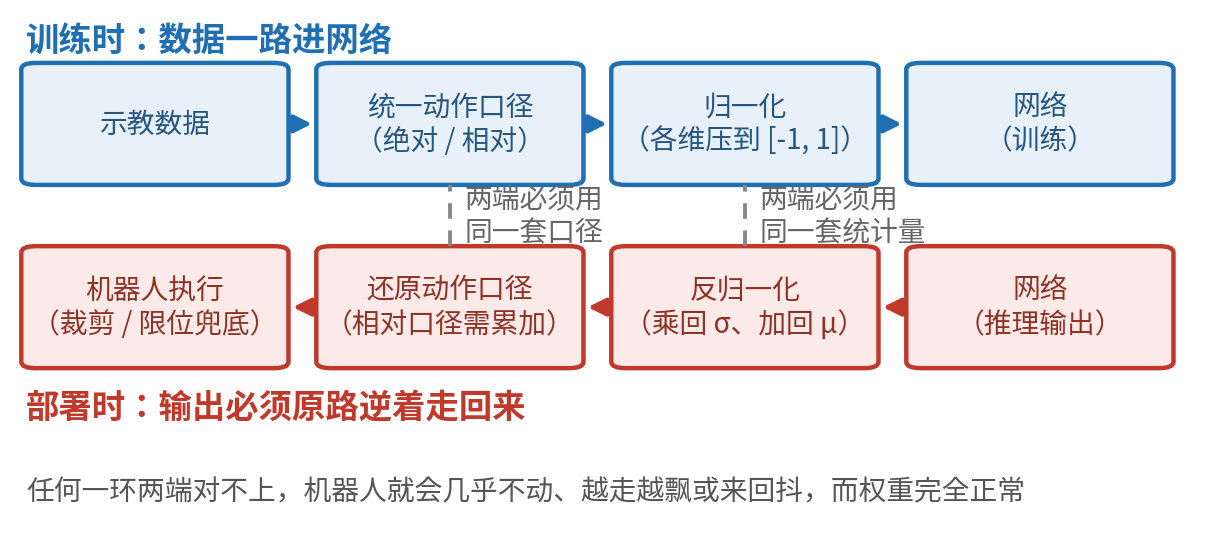
\includegraphics[width=1\linewidth,height=\textheight,keepaspectratio]{../../assets/figures/lecture08/ref/fig08-3-train-deploy-roundtrip.png}

}

\caption{上排是训练时：示教数据先统一动作口径（绝对 /
相对）、再各维归一化，然后进网络；下排是部署时，网络输出沿着\textbf{相反方向}走回来------先反归一化（乘回
σ、加回
μ）、再还原动作口径（相对口径需累加），最后由裁剪限位兜底。中间两条竖虚线标出两处衔接：口径与统计量，两端必须各用同一套（本书自绘）}

\end{figure}%

上图就是本节的路线图。上排画的是训练时数据怎么进网络，下排画的是部署时数据怎么原路走回来；中间那两条虚线，标出了最容易断掉的两处衔接------动作口径（3.3）和归一化统计量（3.4）。在拆这两处衔接之前，先回答一个更基本的问题：怎么判断一个策略到底行不行（3.1、3.2）。

\subsection{3.1
训练损失低不等于任务成功}\label{ux8badux7ec3ux635fux5931ux4f4eux4e0dux7b49ux4e8eux4efbux52a1ux6210ux529f}

最容易踩的认知误区，是盯着训练损失（loss）下降就以为大功告成。

策略的训练目标通常是''让预测动作接近示教动作''，这是一个\textbf{单步}的监督指标。但任务成功是一个\textbf{闭环}的结果：要一步接一步走到底、把方块真的送进容器。单步每步差一点点，几十步累积下来可能完全跑偏；反过来，loss
不是最低的那个
checkpoint，真机成功率反而更高，也很常见。也不存在一个通用的数值，说''loss
降到多少就能部署''------验证集损失、预测动作与示教动作的逐维误差这类\textbf{离线指标}，作用是训练监控、checkpoint
粗筛和故障诊断；最终的任务能力，要在仿真或真机上按统一协议闭环跑一遍才算数。

\begin{quote}
loss
衡量的是''像不像示教''，成功率衡量的是''任务成没成''，两者经常对不上------所以选模型不能只看
loss 曲线。这两类指标是分工，不是互斥：离线筛，闭环定。
\end{quote}

\subsection{3.2 闭环里误差会滚雪球：为什么必须 rollout
验证}\label{ux95edux73afux91ccux8befux5deeux4f1aux6edaux96eaux7403ux4e3aux4ec0ux4e48ux5fc5ux987b-rollout-ux9a8cux8bc1}

为什么单步差一点，闭环会差很多？因为机器人是\textbf{用自己的动作决定自己下一步看到什么}。

训练时策略见到的都是示教里''正确''的状态；一旦它在某一步偏离一点，就进入了训练时没见过的状态，于是下一步预测更偏、状态更陌生------误差像滚雪球一样越滚越大。下图画的就是这个过程：

\begin{figure}[H]

{\centering 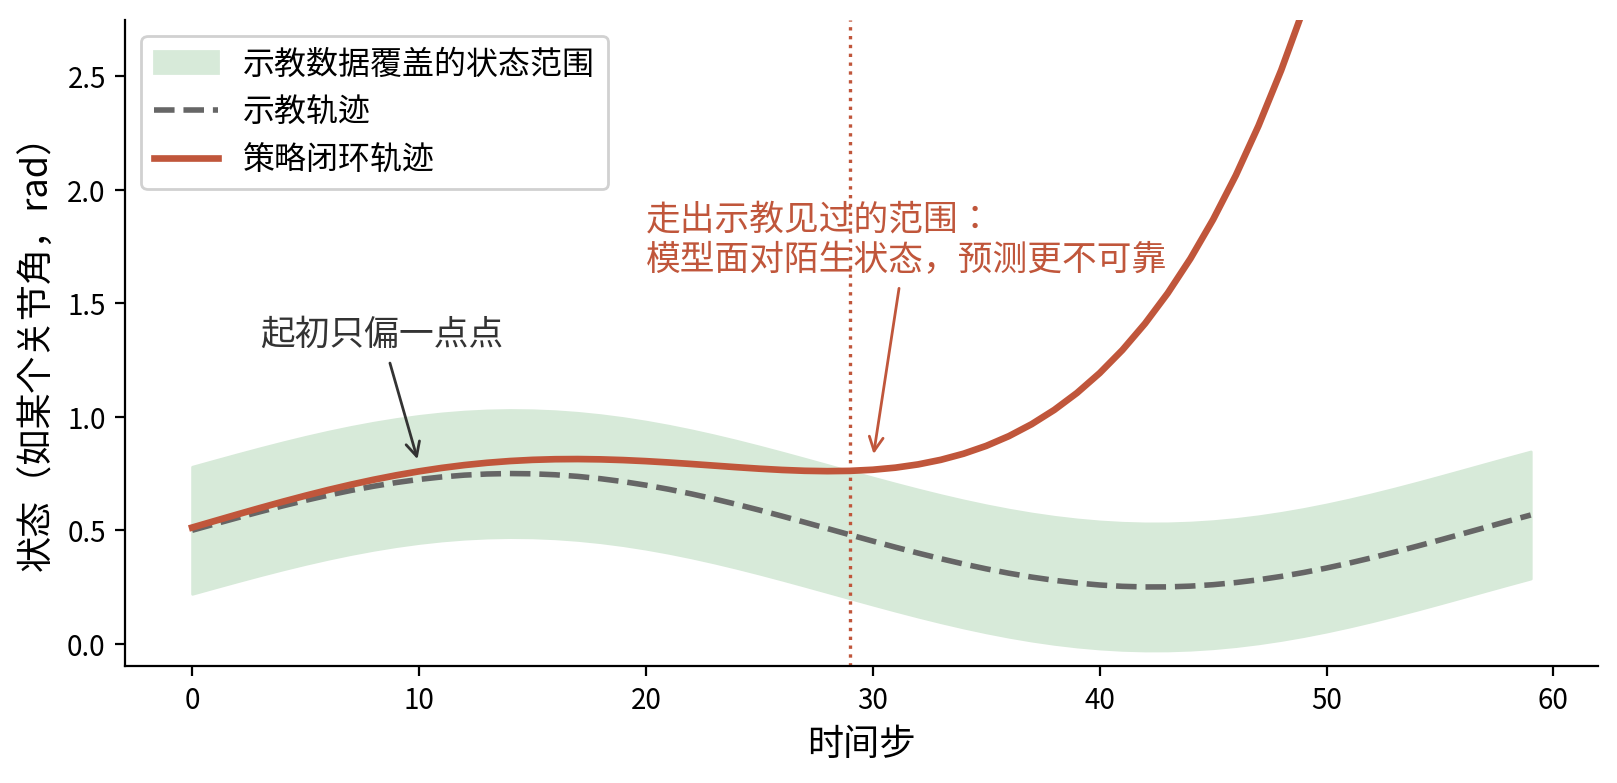
\includegraphics[width=0.85\linewidth,height=\textheight,keepaspectratio]{../../assets/figures/lecture08/ref/832_error-snowball.png}

}

\caption{绿色带是示教数据覆盖过的状态范围；策略的闭环轨迹起初只比示教偏一点点，一旦走出绿色带、进入模型没见过的状态，预测越来越不可靠，误差加速放大}

\end{figure}%

注意图里的转折点：轨迹还在绿色带内时，偏差几乎看不出来；\textbf{走出带子的那一刻}，模型面对的是示教里从未出现过的状态，输出开始失去依据，轨迹加速飘走。这个现象叫\textbf{分布漂移}（distribution
shift）；在模仿学习里它有个更精确的名字叫\textbf{协变量偏移}（covariate
shift），指的正是''策略自己走出来的状态分布''和''示教数据的状态分布''对不上。它是模仿学习的经典难题，Ross
等人提出的 \textbf{DAgger}{[}7{]}（数据聚合，Dataset
Aggregation：让策略先跑，再请专家对跑出来的状态补标正确动作，把这批数据加回训练集重训）就是冲它去的。第10讲
1.2 节会从生成式策略的角度再碰一次这个问题，DAgger
这条交互式纠正的路，则留到第16讲 8.6 节的人在环方法展开。

结论很硬：\textbf{策略到底行不行，得让它在环境里真正跑一遍（rollout）、看任务成没成------离线指标做不了这个判决。}
离线指标仍然有它的位置：粗筛
checkpoint、诊断故障、在上真机之前先把明显的问题挡掉，从而降低真机风险。这也是为什么本讲第
4 节的实验，核心不是算 loss，而是让策略在仿真里闭环跑起来。

\subsection{3.3
动作口径：绝对还是相对，两端必须说同一种话}\label{ux52a8ux4f5cux53e3ux5f84ux7eddux5bf9ux8fd8ux662fux76f8ux5bf9ux4e24ux7aefux5fc5ux987bux8bf4ux540cux4e00ux79cdux8bdd}

2.2 提过动作可以是\textbf{绝对}的，也可以是\textbf{相对}的（增量 /
delta）。这是这一讲最该记牢的细节之一------它既影响网络好不好学，又是部署时最常翻车的地方。

先把两种口径说清楚。假设机械臂某个关节此刻在 1.18
弧度，下一帧示教把它转到了 1.20 弧度，那么''这一步动作''有两种记法：

\begin{figure}[H]

{\centering 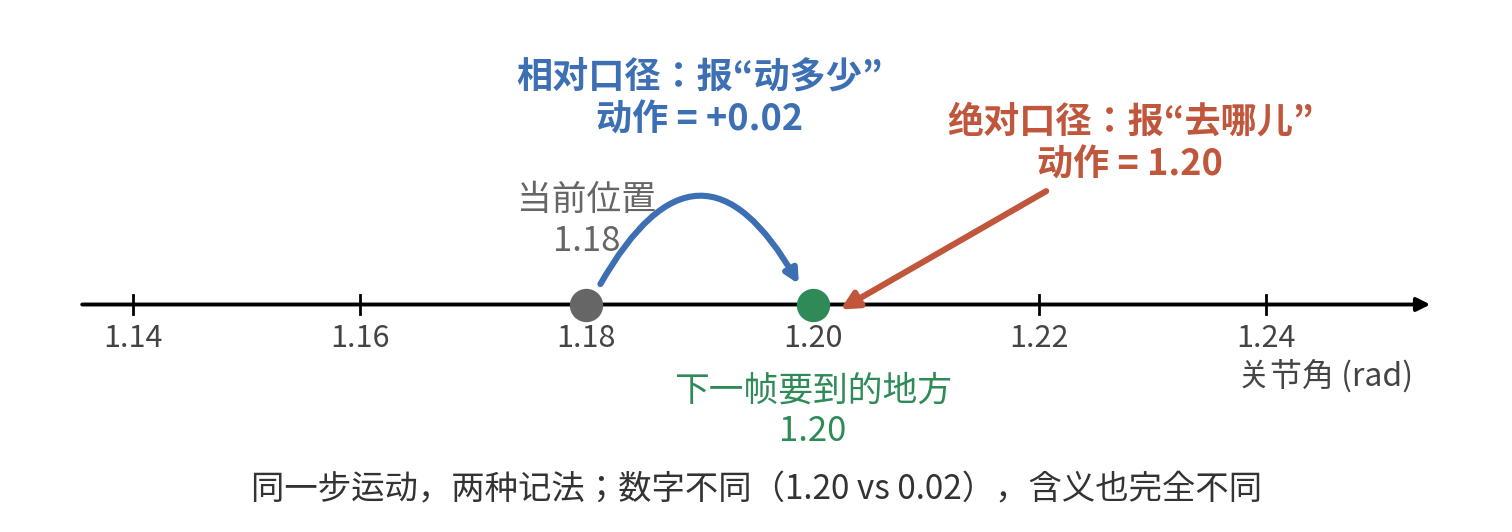
\includegraphics[width=0.8\linewidth,height=\textheight,keepaspectratio]{../../assets/figures/lecture08/ref/833_abs-vs-delta-axis.png}

}

\caption{同一步运动的两种记法：相对口径报''动多少''（+0.02），绝对口径报''去哪儿''（1.20）；数字不同，含义也完全不同（本书自绘；三个数的来源是上面那个
1.18 转到 1.20 的算例）}

\end{figure}%

\begin{itemize}
\tightlist
\item
  \textbf{绝对口径}：策略直接输出''目标 = 1.20
  弧度''。动作的含义是\textbf{去哪儿}，跟你现在在哪没关系。
\item
  \textbf{相对口径}：策略输出''在当前基础上 +0.02
  弧度''。动作的含义是\textbf{动多少}，必须配合''当前在哪''才能还原出真正的目标（\(1.18 + 0.02 = 1.20\)）。
\end{itemize}

末端位姿也是一样：可以给''末端在世界坐标系下的绝对位姿''，也可以给''末端再往前挪
1
厘米''这种增量。两种口径各有长短，没有绝对的好坏：绝对口径每一步都瞄准一个固定坐标，动作表示本身不会累积漂移，但网络得记住''整个工作空间长什么样''；相对口径是''局部修正''，跨起点泛化好、通常也更好学，代价是部署时要一步步把增量累加回绝对位置。口径的选择本身就影响性能------Diffusion
Policy
那篇论文专门做过这项对照{[}8{]}：方法完全不变，只把动作表示从速度口径换成位置口径，多个任务上的成功率就明显不同。

真正的分水岭在于：\textbf{训练和部署两端，必须用同一种口径去解释同一个数字。}
这里要留意相对口径的一个数值特点：增量的绝对值天然很小。粗算一下就知道------采集频率
30Hz、关节以每秒零点几弧度这种温和速度转动，相邻两帧之间就只差 0.01
弧度上下，几乎贴着 0。由此引出两个对称的坑，下图左右各画了一个：

\begin{figure}[H]

{\centering \pandocbounded{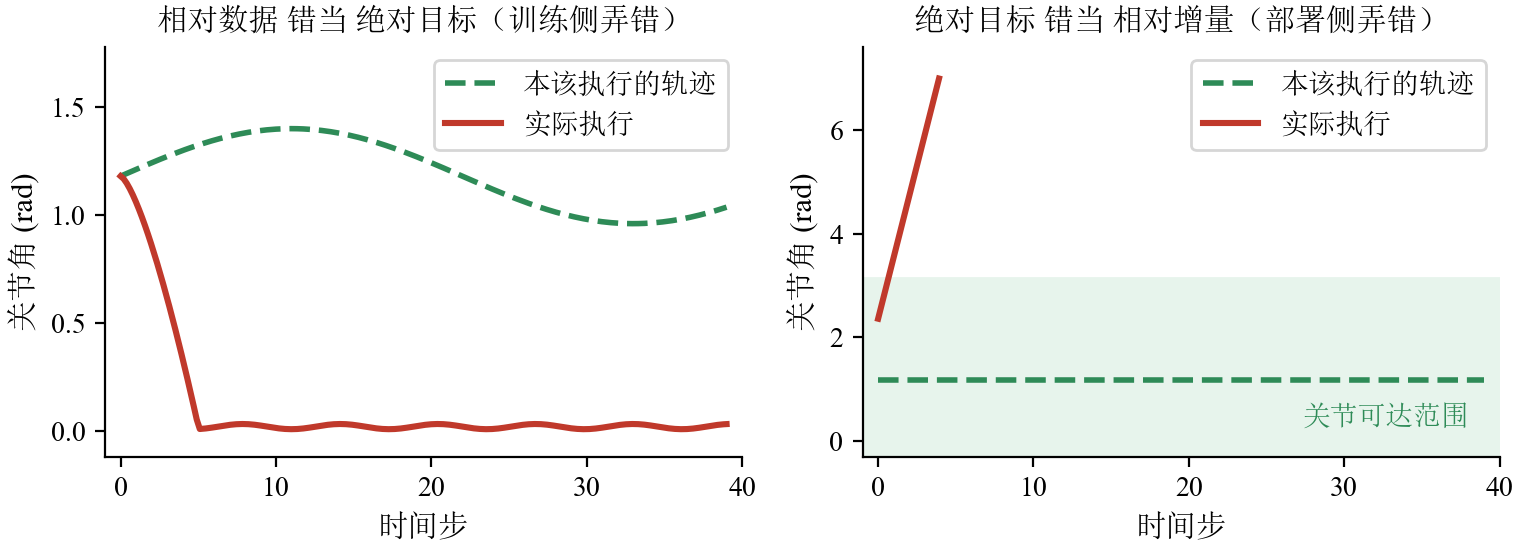
\includegraphics[keepaspectratio]{../../assets/figures/lecture08/ref/833_mismatch-failures.png}}

}

\caption{左：相对数据被错当成绝对目标训练，网络学会输出''绝对目标约等于
0''，机械臂扎向零位后几乎不动；右：绝对目标被错当成相对增量部署，每步都在当前位置上再累加，关节角一路冲出可达范围}

\end{figure}%

\begin{itemize}
\tightlist
\item
  \textbf{左图，训练侧弄错------把相对数据当绝对目标训}：本该是''+0.02''的增量，被错当成绝对目标喂给网络。网络于是学会''不管现在在哪，都输出一个
  0.02
  左右的绝对目标''------机械臂径直扎向接近零位的姿态。到了那儿之后，每一步给出的目标几乎都是同一个数，机械臂原地不动；那点残余的位移比网络的预测噪声还小，看上去就是在抖。症状：\textbf{先猛地一动，然后几乎不动}。此时
  loss 依然很漂亮、网络本身也没毛病，机器人却罢工了。
\item
  \textbf{右图，部署侧弄错------把绝对目标当相对增量发}：训练时动作是绝对目标（比如
  1.2），部署端却把它当成增量，每步都在当前位置上再加
  1.2------关节角一路累加、冲出可达范围。症状：\textbf{单调地越走越远}（发散）。反过来，相对模型部署时忘了''目标
  = 当前位置 + 增量''这步累加，把 0.02
  直接当绝对目标下发，就回到左图的下场。
\end{itemize}

\begin{quote}
备注：动作口径必须在训练和部署两端\textbf{完全一致}------同一个数字
0.02，在绝对口径下意思是''去 0.02 弧度处''，在相对口径下意思是''再走
0.02
弧度''，差之毫厘谬以千里。这是一条约定层面的硬约束，不是事后调参能补救的。
\end{quote}

\begin{quote}
备注：口径的约定其实从\textbf{采数据}那一刻就开始了。主从遥操作里从臂跟随主臂，也分两种方式------\textbf{绝对跟踪}：从臂直接去主臂当前的绝对姿态，录下的动作就是从臂真实到达的姿态，前提是主从标定的零点对齐；\textbf{相对（锚定）跟踪}：接通的第一帧记下''从臂当前姿态减主臂姿态''的差，之后从臂只复现主臂的位移。锚定跟踪不要求零点严格对齐、接通瞬间从臂不会突然跳动，但录下的动作和从臂实际姿态恒差一个\textbf{每次开机都不同的常数}------动作口径已经被悄悄改写，部署时更容易两端对不上。遥操作采数据的细节，下一讲展开。
\end{quote}

\subsection{3.4
归一化：把统计量和模型绑在一起}\label{ux5f52ux4e00ux5316ux628aux7edfux8ba1ux91cfux548cux6a21ux578bux7ed1ux5728ux4e00ux8d77}

第二处容易断掉的衔接是\textbf{归一化}（normalization）------把不同量纲的数值统一缩放到相近的区间。

\textbf{为什么非归一化不可。}
一份机器人数据里，不同物理量的数值范围天差地别：关节角可能在
\([-3.14, 3.14]\)、夹爪开合是 \([0, 1]\)、图像像素是
\([0, 255]\)。神经网络对数值尺度很敏感，所以训练前几乎都会把每一维\textbf{各自}归一化到相近的尺度。这里要分两头说，因为它们解决的是两件不同的事：

\begin{itemize}
\tightlist
\item
  \textbf{输入侧（图像、状态）归一化}改善数值条件，并且要和视觉编码器预训练时用的那套归一化对上------很多模型直接沿用预训练编码器固定的
  mean/std，不能自己另算一套。
\item
  \textbf{动作侧（输出）归一化}才是''平衡各维度''那件事：动作各维共用一个回归/生成损失，量程大的维度会主导这个损失、量程小的维度几乎学不动。
\end{itemize}

两头的统计量、变换和反变换都必须\textbf{分别}记录，别混成一套。

\begin{figure}[H]

{\centering 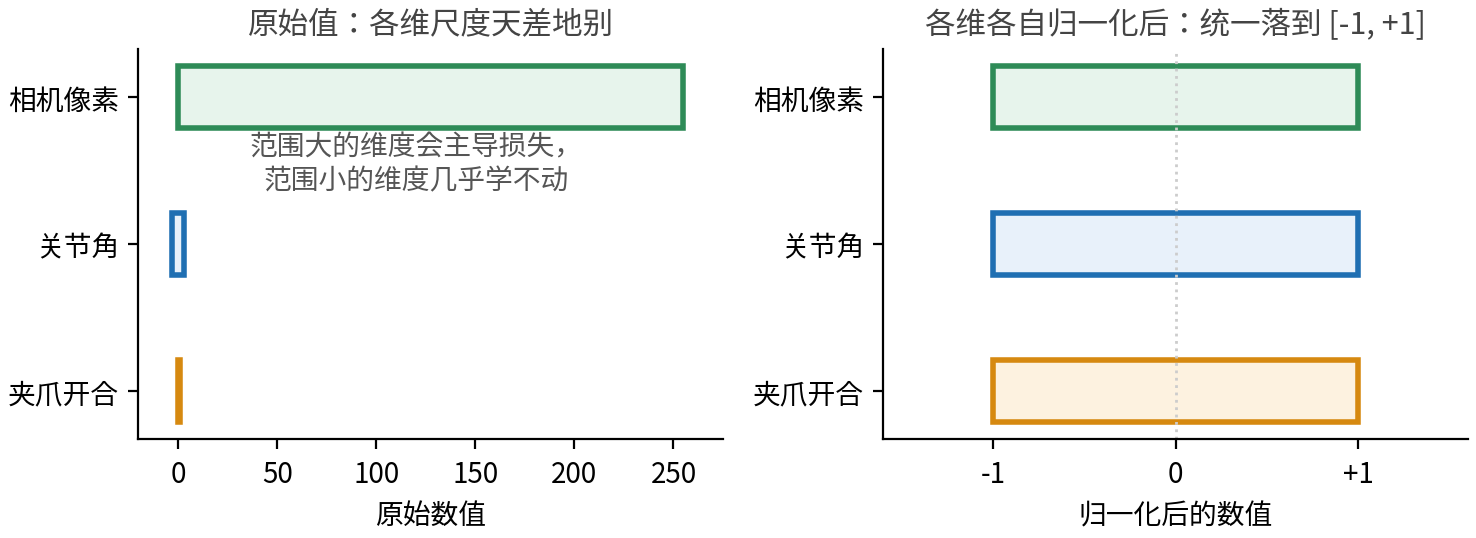
\includegraphics[width=1\linewidth,height=\textheight,keepaspectratio]{../../assets/figures/lecture08/ref/fig08-3-normalization-ranges.png}

}

\caption{左：相机像素、关节角、夹爪开合三种量的原始数值范围相差悬殊；右：各维各自归一化后，统一落到
{[}-1, +1{]}（本书自绘）}

\end{figure}%

左图里关节角和夹爪开合那两条几乎看不见的细条就是问题所在：\([-3.14, 3.14]\)
和 \([0, 1]\) 摆在 0 到 255
的像素旁边，被压成了两道竖线。右图三条一样长------归一化要做的不是把数值改小，而是把各维放到同一把尺子上。

常见两种做法。第一种是\textbf{均值-方差（mean /
std）}：\(\hat{x} = (x - \mu) / \sigma\)，用这一维的均值 \(\mu\)
和标准差 \(\sigma\)
把数据拉成零均值、单位方差。简单，但对离群点敏感------数据里混进几个异常大的值（比如传感器毛刺），\(\sigma\)
就被撑大，正常值反而被压扁。

第二种是\textbf{分位数（q01 / q99）}。先说清 q99
是什么：把这一维的所有数据\textbf{从小到大排队，排在 99\%
位置上的那个数就是 q99}------也就是说，99\% 的数据都不超过它；q01
同理，是排在 1\% 位置上的数。归一化时不用最小值和最大值，而用
\([q_{01}, q_{99}]\) 这段区间做线性缩放，把它映射到
\([-1, +1]\)；落在区间外的样本直接截断到边界上------注意是\textbf{两端各约
1\%、合计约 2\%}（\(q_{01}\) 以下约 1\%，\(q_{99}\) 以上约
1\%），实际比例还受重复值和具体实现影响：

\begin{figure}[H]

{\centering \pandocbounded{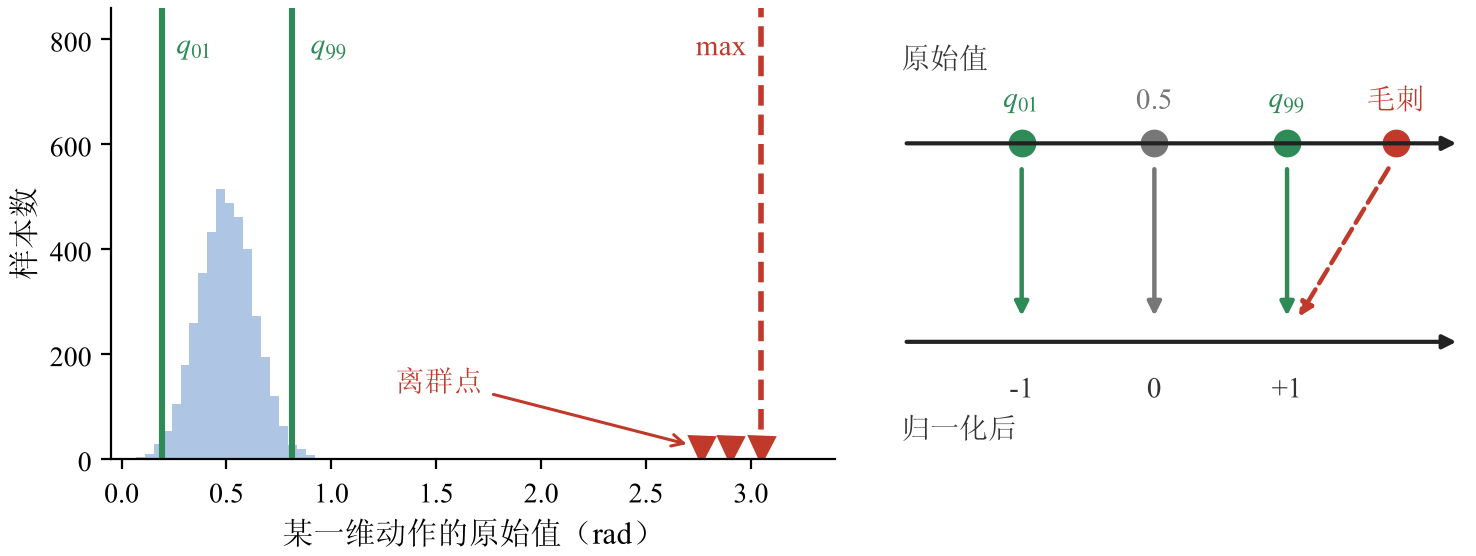
\includegraphics[keepaspectratio]{../../assets/figures/lecture08/ref/834_q99-normalization.png}}

}

\caption{左：直方图里几个离群点把 max 拉得很远，而 q01/q99
紧贴数据主体；右：把 {[}q01, q99{]} 线性映射到 {[}-1, +1{]}，超出 q99
的毛刺被截断到 +1}

\end{figure}%

好处在左图一眼可见：min / max 会被那几个毛刺整个带偏，q01 / q99
则稳稳贴住数据主体。所以分位数归一化更抗离群点。

但\textbf{不要把它当成放之四海的默认值}------连同一个系列的两代模型都不一样。把
LeRobot v0.5.1 里几个常用策略的默认归一化摊开看：

\begin{center}
\begin{tabular}{@{}>{\raggedright\arraybackslash}p{\dimexpr 0.3750\linewidth - 2\tabcolsep\relax} >{\raggedright\arraybackslash}p{\dimexpr 0.1719\linewidth - 2\tabcolsep\relax} >{\raggedright\arraybackslash}p{\dimexpr 0.1719\linewidth - 2\tabcolsep\relax}@{}}
\toprule\noalign{}
策略（LeRobot v0.5.1） & 状态侧 & 动作侧 \\
\midrule\noalign{}
\(\pi_0\) & 均值-方差 & 均值-方差 \\
\(\pi_{0.5}\) & 分位数 & 分位数 \\
ACT & 均值-方差 & 均值-方差 \\
Diffusion Policy & 最小-最大 & 最小-最大 \\
SmolVLA & 均值-方差 & 均值-方差 \\
\bottomrule\noalign{}
\end{tabular}
\end{center}

分位数确实被用了，但用它的是 \(\pi_{0.5}\)；\(\pi_0\)
自己走的还是均值-方差。\(\pi_0\) 的官方实现 openpi
里也是同一个口径：分位数归一化那个开关对 \(\pi_0\) 是显式关掉的，从
\(\pi_{0.5}\)
起才打开。每个策略都在自己的配置里分别声明图像、状态、动作三路各用哪种归一化（上表只列了状态与动作两路），换策略、换版本都要回去看一眼实际用的是哪种------照搬别处的假设，就是这一节剩下要讲的那类翻车。

举个具体的数走一遍归一化的''来回''。某关节在训练集上统计出
\(\mu = 0.3\)、\(\sigma = 0.5\)。示教里一个目标 0.8，归一化后是
\((0.8 - 0.3)/0.5 = 1.0\)，网络学到的、吐出来的都是这个
1.0。轮到推理时网络输出
1.0，必须再\textbf{反归一化}回真实尺度：\(1.0 \times 0.5 + 0.3 = 0.8\)，这个
0.8
才是真正下发给机器人的值。训练（正向归一化）和部署（反向还原）用的，必须是同一套
\(\mu, \sigma\)。

\textbf{关键在于：这套统计量（\(\mu, \sigma\) 或 q01 /
q99）是从训练集统计出来的，是模型的一部分}------它通常和权重放在一起，存成一个不起眼的小文件。部署时如果只带走了权重、把统计量落下了，或者拿错成另一份数据（另一个
\texttt{asset\_id}）的统计量，那就是一个\textbf{部署错误}，应当当场暴露出来。别指望框架会好心地帮你兜住。不同实现在这件事上的行为并不一致：有的直接报错停下，有的则悄悄回退到一套默认值、或者加载另一份资产接着跑。后一种最危险------本该还原成
0.8 的动作被原样当成 1.0
发了出去，日志里一句提示都没有。所以启动时就要校验统计量的键、维度、版本和数值范围，\textbf{禁止静默回退}；否则整条动作的尺度会系统性错位，而你只看到下图这两种症状：

\begin{figure}[H]

{\centering 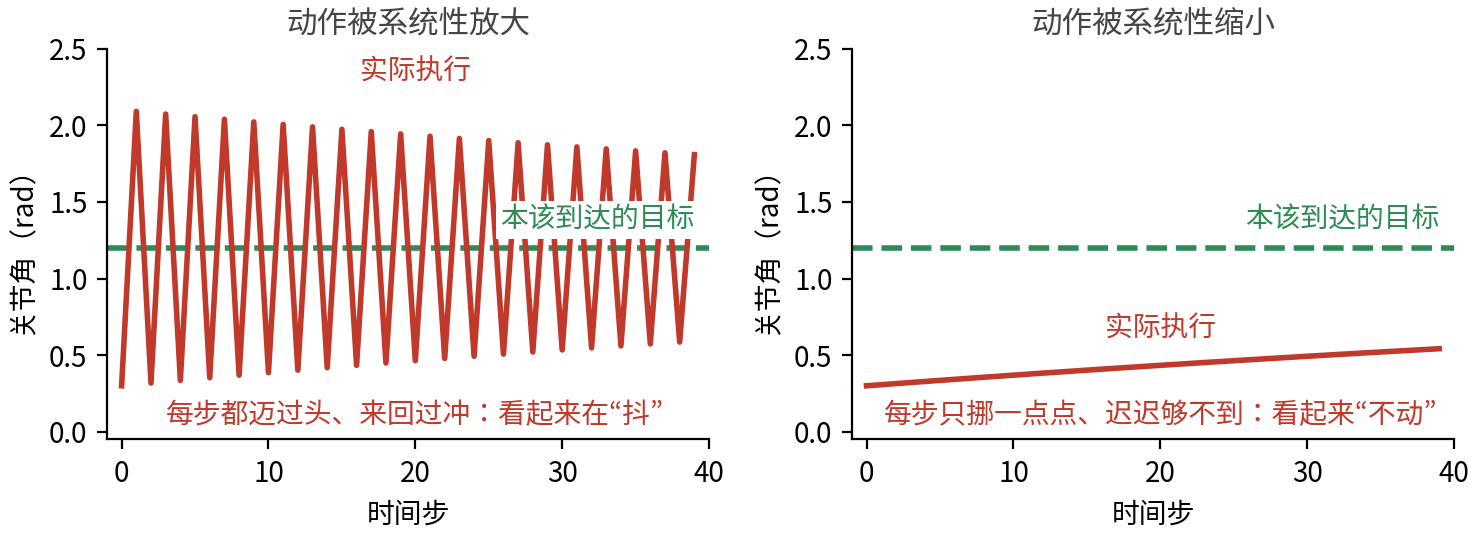
\includegraphics[width=1\linewidth,height=\textheight,keepaspectratio]{../../assets/figures/lecture08/ref/fig08-3-scale-error-symptoms.png}

}

\caption{左：动作被系统性放大，每步都迈过头、围绕目标来回过冲，看起来在''抖''；右：动作被系统性缩小，每步只挪一点点、迟迟够不到目标，看起来''不动''。两图里绿色虚线都是本该到达的目标（本书自绘）}

\end{figure}%

两条红线的形状本身就是诊断依据：左图围着绿线上下穿行，幅度只是缓慢收窄，四十步都没停下来；右图是一条单调的缓坡，四十步走完还不到目标距离的三分之一。这种错和
3.3
的坑同一个性质：网络、权重都没问题，全错在''模型和它的附属统计量分了家''。

\begin{quote}
一句话：模型权重和它的归一化统计量是\textbf{一套}东西；权重对了、统计量丢了或拿错了，输出照样全错。而且观测侧（输入）和动作侧（输出）两头都要归一化，部署时两套统计量一个都不能少------启动时先校验，别等机器人动起来才发现。
\end{quote}

\subsection{3.5
裁剪、限位与出发前检查单}\label{ux88c1ux526aux9650ux4f4dux4e0eux51faux53d1ux524dux68c0ux67e5ux5355}

就算前面都对，真机上还要留一道兜底闸：把动作\textbf{裁剪}（clip）到合理范围、限制最大速度、加上关节限位。策略偶尔吐出一个离谱的值时，这道闸能把它拦在幅值之内。但要清楚它的能力边界：裁剪只管\textbf{单次}幅值，管不了轨迹整体------连续多个贴着边界的动作、坐标系搞错、绝对/相对口径搞反，照样能做出危险运动。所以它是\textbf{最低层的数值保护}，上面还要叠加一层层约束：限加速度、限加加速度（jerk，也就是加速度的变化率，管的是动作平不平顺），再加上工作空间约束、碰撞监测、看门狗、急停，以及先低速分阶段验证、确认没问题再放速度。

最后，把本节的内容收成一张\textbf{出发前检查单}，部署前逐行过一遍：

\begin{center}
\begin{tabular}{@{}>{\raggedright\arraybackslash}p{\dimexpr 0.1421\linewidth - 2\tabcolsep\relax} >{\raggedright\arraybackslash}p{\dimexpr 0.8579\linewidth - 2\tabcolsep\relax}@{}}
\toprule\noalign{}
检查项 & 要确认的问题 \\
\midrule\noalign{}
动作口径 & 训练数据的动作是绝对还是相对？部署端按同一种口径解释了吗（相对口径记得累加还原）？ \\
归一化统计量 & 统计量文件和权重在一起吗？观测侧、动作侧两套都齐吗？ \\
数值量级 & 离线喂几帧观测，输出的数值量级像正常动作吗（相对口径应是贴近 0 的小数）？ \\
起始位姿 & 机器人从示教数据里出现过的起始位姿附近出发了吗？ \\
安全兜底 & 裁剪、限速、关节限位这道闸设了吗？加速度限制、工作空间、碰撞监测、看门狗、急停齐了吗？ \\
评估标准 & 判好坏的标准定成 rollout 成功率了吗（而不是 loss）？ \\
\bottomrule\noalign{}
\end{tabular}
\end{center}

这张表不长，但每一行背后都是一类''模型没毛病、机器人不工作''的故障。第 4
节的实验会拿着它逐行核对一遍。

\subsection{3.6 本节小结}\label{ux672cux8282ux5c0fux7ed3-1}

把一个策略从训练搬到部署，本质是让数据把那条''来回路''走完整：训练侧怎么把示教数据变换进网络（统一动作口径、归一化），部署侧就必须用同一套约定逆着变换回来（反归一化、还原口径），最后用裁剪与限位兜底；判断成没成，只认闭环
rollout（3.1、3.2）。这些都不是算法创新，却是机器人能不能动起来的分水岭------``模型看着没问题、就是不工作''的故障，十有八九断在来回路的某一环上，症状无非三种：不动、发散、抖动。

\section{\texorpdfstring{4 实验：用 \(\pi_0\)
跑通第一个策略闭环}{4 实验：用 \textbackslash pi\_0 跑通第一个策略闭环}}\label{ux5b9eux9a8cux7528-pi_0-ux8dd1ux901aux7b2cux4e00ux4e2aux7b56ux7565ux95edux73af}

讲了这么多概念，这一节亲手跑一个真正的策略，把''看一眼、动一下''的闭环看在眼里。我们用一个现成的、能力很强的
VLA------\textbf{\(\pi_0\)}------当作黑盒策略，在仿真环境 LIBERO
里跑一遍 rollout。

这里有个容易踩的前提要先说清楚：\textbf{用的不是 \(\pi_0\)
的通用基座权重，而是一份已经在 LIBERO 上微调过的 checkpoint}。\(\pi_0\)
的基座预训练数据里不含 LIBERO 仿真数据，直接零样本丢进 LIBERO
是跑不出成功率的------必须配上对应的 LIBERO
微调配置与权重。本讲实验固定用 LeRobot 提供的
\texttt{lerobot/pi0\_libero\_finetuned\_v044}（代码见
\texttt{code/vla/1\_policy\_rollout/1\_2\_pi0\_libero\_rollout/pi0\_demo.py}）；openpi
那条线上对应的是 \texttt{pi0\_libero} 配置与
checkpoint------同一个仓库里还并列着
\texttt{pi0\_fast\_libero}、\texttt{pi05\_libero}
这些名字很像的变体，它们背后是不同的模型，别拿错。换版本要连着配置、归一化资产、评测脚本一起换，不能只换权重文件。

\subsection{\texorpdfstring{4.1 先认识主角：\(\pi_0\)
当一个黑盒策略}{4.1 先认识主角：\textbackslash pi\_0 当一个黑盒策略}}\label{ux5148ux8ba4ux8bc6ux4e3bux89d2pi_0-ux5f53ux4e00ux4e2aux9ed1ux76d2ux7b56ux7565}

\(\pi_0\) 是 Physical Intelligence
提出的视觉-语言-动作模型{[}9{]}：一个视觉-语言骨干网络看懂图像和指令，后面接一个''动作专家''生成连续动作。

\begin{figure}[H]

{\centering \pandocbounded{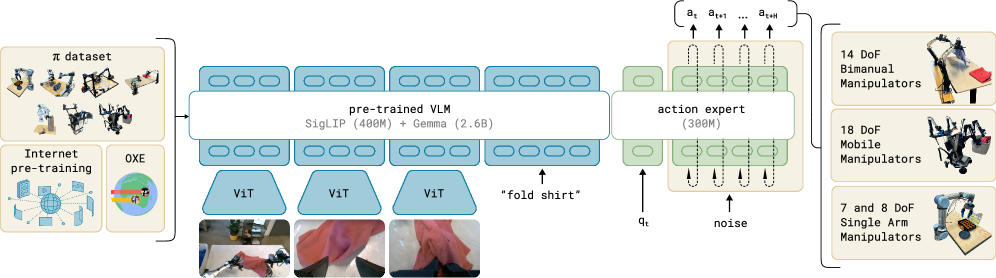
\includegraphics[keepaspectratio]{../../assets/figures/lecture08/ref/841_pi0-architecture_arxiv-2410.24164.png}}

}

\caption{\(\pi_0\)
框架总览：视觉-语言骨干处理图像与语言指令，较小的动作专家以连续方式输出机器人动作}

\end{figure}%

\begin{quote}
备注：\(\pi_0\) 内部用 flow matching 生成动作，这套机制留到第10讲 5
节（Flow Matching）和第11讲 3
节（\(\pi_0\)）再拆。\textbf{本讲只把它当一个''观测进、动作出''的黑盒}------恰好印证第
2 节对策略的定义。
\end{quote}

\subsection{4.2 搭好舞台：LIBERO
仿真环境}\label{ux642dux597dux821eux53f0libero-ux4effux771fux73afux5883}

LIBERO{[}10{]}
是一个机器人操作的仿真基准，用程序化的方式生成了一批桌面操作任务，分成空间、物体、目标、长程四个套件。没有真机时，它就是我们验证策略的标准台子：

\begin{figure}[H]

{\centering \pandocbounded{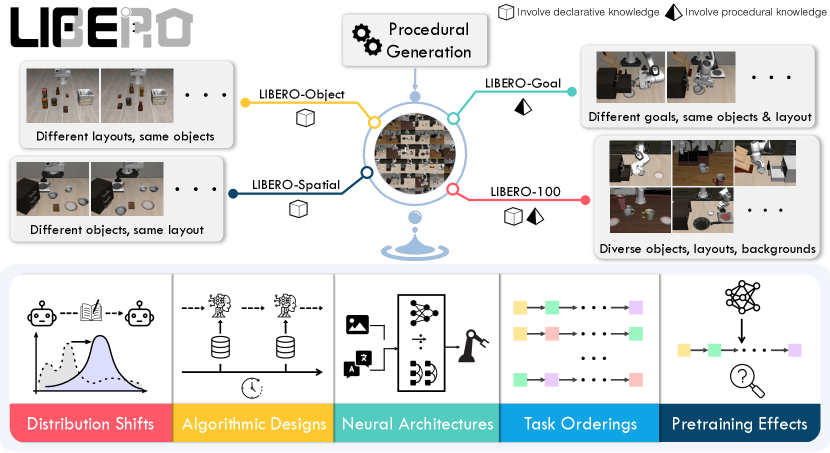
\includegraphics[keepaspectratio]{../../assets/figures/lecture08/ref/842_libero-task-suites_arxiv-2306.03310.png}}

}

\caption{LIBERO 程序化生成的四个任务套件：空间、物体、目标与长程}

\end{figure}%

在跑策略之前，先花几分钟把这个环境本身摸清楚------观测里有什么、动作是几维、发一个动作末端会往哪动。这三件事正是
2.2 节那两个接口在一个具体环境里的样子。完整脚本在
\texttt{code/vla/1\_policy\_rollout/1\_1\_libero\_env/libero\_demo.py}，建一个环境只要这几行：

\begin{Shaded}
\begin{Highlighting}[]
\NormalTok{env\_cfg }\OperatorTok{=}\NormalTok{ LiberoEnvConfig(}
\NormalTok{    task}\OperatorTok{=}\StringTok{"libero\_spatial"}\NormalTok{,}
\NormalTok{    task\_ids}\OperatorTok{=}\NormalTok{[}\DecValTok{0}\NormalTok{],}
\NormalTok{    obs\_type}\OperatorTok{=}\StringTok{"pixels\_agent\_pos"}\NormalTok{,   }\CommentTok{\# 图像 + 本体状态 两路观测}
\NormalTok{    observation\_height}\OperatorTok{=}\DecValTok{256}\NormalTok{,}
\NormalTok{    observation\_width}\OperatorTok{=}\DecValTok{256}\NormalTok{,}
\NormalTok{)}

\NormalTok{envs }\OperatorTok{=}\NormalTok{ make\_env(env\_cfg, n\_envs}\OperatorTok{=}\DecValTok{1}\NormalTok{)}
\NormalTok{env  }\OperatorTok{=}\NormalTok{ envs[}\StringTok{\textquotesingle{}libero\_spatial\textquotesingle{}}\NormalTok{][}\DecValTok{0}\NormalTok{]}
\end{Highlighting}
\end{Shaded}

\texttt{obs\_type="pixels\_agent\_pos"}
这一个参数就把观测的口径定死了：图像一路、本体状态一路。换成别的取值，策略拿到的观测就变了------而策略的输入接口是训练时就固定下来的，对不上就跑不了。

动作那一头同样要当场确认，不要靠猜：

\begin{Shaded}
\begin{Highlighting}[]
\NormalTok{action\_space }\OperatorTok{=}\NormalTok{ env.single\_action\_space}
\BuiltInTok{print}\NormalTok{(}\SpecialStringTok{f"Action space: }\SpecialCharTok{\{}\NormalTok{action\_space}\SpecialCharTok{\}}\SpecialStringTok{"}\NormalTok{)}
\ControlFlowTok{assert}\NormalTok{ action\_space.shape }\OperatorTok{==}\NormalTok{ (}\DecValTok{7}\NormalTok{,)}
\end{Highlighting}
\end{Shaded}

7 维，就是 4.5 节要核对的那个动作口径。这句 \texttt{assert}
值得留着：环境版本一变，维度对不上会当场炸，总好过让一个维度错位的动作悄悄发到机器人上。

\subsection{4.3
闭环跑起来：看一眼、动一下}\label{ux95edux73afux8dd1ux8d77ux6765ux770bux4e00ux773cux52a8ux4e00ux4e0b}

实验的核心是一个循环：从环境拿到当前观测（相机图 + 机器人状态 +
语言指令）→ 喂给 \(\pi_0\) → 得到一段动作 → 在环境里执行 →
拿到新的观测\ldots\ldots 如此往复，直到任务完成或超时。这就是第 3
节反复强调的\textbf{闭环
rollout}：策略不是预测一次就完事，而是要在自己造成的后果里一直走下去。

代码在
\texttt{code/vla/1\_policy\_rollout/1\_2\_pi0\_libero\_rollout/pi0\_demo.py}。第一步是把策略连同它的归一化统计量一起加载进来：

\begin{Shaded}
\begin{Highlighting}[]
\NormalTok{    policy\_path }\OperatorTok{=} \StringTok{"lerobot/pi0\_libero\_finetuned\_v044"}
\NormalTok{    policy\_cfg }\OperatorTok{=}\NormalTok{ PreTrainedConfig.from\_pretrained(policy\_path)}
\NormalTok{    policy\_cfg.device }\OperatorTok{=} \StringTok{"cuda"} \ControlFlowTok{if}\NormalTok{ torch.cuda.is\_available() }\ControlFlowTok{else} \StringTok{"cpu"}
\NormalTok{    policy }\OperatorTok{=}\NormalTok{ get\_policy\_class(policy\_cfg.}\BuiltInTok{type}\NormalTok{).from\_pretrained(}
\NormalTok{        policy\_path, config}\OperatorTok{=}\NormalTok{policy\_cfg, strict}\OperatorTok{=}\VariableTok{False}
\NormalTok{    )}
\NormalTok{    preprocessor, postprocessor }\OperatorTok{=}\NormalTok{ make\_pre\_post\_processors(policy\_cfg, pretrained\_path}\OperatorTok{=}\NormalTok{policy\_path)}
\end{Highlighting}
\end{Shaded}

最后那行是 3.4 节的主角落到代码上的样子。\texttt{preprocessor}
做正向归一化，\texttt{postprocessor} 做反归一化，两者的统计量都从
\texttt{policy\_path}
这一个来源读出来------统计量和权重同进同出，不会分家。如果哪天你写的推理脚本里只有
\texttt{from\_pretrained}
而没有这一行，那就是把归一化整个跳过了，动作尺度会系统性错位。

装好之后，闭环本身只有十来行：

\begin{Shaded}
\begin{Highlighting}[]
        \ControlFlowTok{for}\NormalTok{ \_ }\KeywordTok{in} \BuiltInTok{range}\NormalTok{(max\_steps):}
\NormalTok{            observation\_batch }\OperatorTok{=}\NormalTok{ preprocess\_observation(observation)}
\NormalTok{            observation\_batch }\OperatorTok{=}\NormalTok{ add\_envs\_task(env, observation\_batch)}
\NormalTok{            observation\_batch }\OperatorTok{=}\NormalTok{ env\_preprocessor(observation\_batch)}
\NormalTok{            observation\_batch }\OperatorTok{=}\NormalTok{ preprocessor(observation\_batch)}

            \ControlFlowTok{with}\NormalTok{ torch.inference\_mode():}
\NormalTok{                action }\OperatorTok{=}\NormalTok{ policy.select\_action(observation\_batch)}

\NormalTok{            action }\OperatorTok{=}\NormalTok{ postprocessor(action)}
\NormalTok{            action }\OperatorTok{=}\NormalTok{ env\_postprocessor(\{}\StringTok{"action"}\NormalTok{: action\})[}\StringTok{"action"}\NormalTok{].cpu().numpy()}

\NormalTok{            observation, \_, terminated, truncated, info }\OperatorTok{=}\NormalTok{ env.step(action)}
\NormalTok{            frames.append(env.envs[}\DecValTok{0}\NormalTok{].render())}
\end{Highlighting}
\end{Shaded}

把它对着第 3
节那张来回路的图读一遍，每一行都能找到位置：四行预处理是''去路''，\texttt{select\_action}
是网络本身，两行后处理是''回程''（先反归一化、再还原成环境的动作口径），\texttt{env.step}
把动作作用回环境、换来下一帧观测。第 2 节说策略是一个 \(a = \pi(o)\)
的函数，在这里就是中间那两行；剩下的全是在给这个函数配上正确的输入输出口径。

一段成功的 rollout 会被写成模块目录下的
\texttt{output/pi0\_libero\_success.mp4}。脚本在写视频之前先拦了两道：

\begin{Shaded}
\begin{Highlighting}[]
        \ControlFlowTok{if} \KeywordTok{not}\NormalTok{ frames:}
            \ControlFlowTok{raise} \PreprocessorTok{RuntimeError}\NormalTok{(}\StringTok{"no frames"}\NormalTok{)}
        \ControlFlowTok{if} \KeywordTok{not}\NormalTok{ success:}
            \ControlFlowTok{raise} \PreprocessorTok{RuntimeError}\NormalTok{(}\StringTok{"no success"}\NormalTok{)}
\end{Highlighting}
\end{Shaded}

这两行不是防御性编程的样板，而是 3.1
节那条结论的代码版：\textbf{跑完不等于跑对}。没有它们，一次''程序正常退出但任务没完成''的运行看起来和成功没有区别------而这恰恰是本讲反复强调的那类故障的样子。

跑通之后那段视频抽成四帧，长这样：

\begin{figure}[H]

{\centering 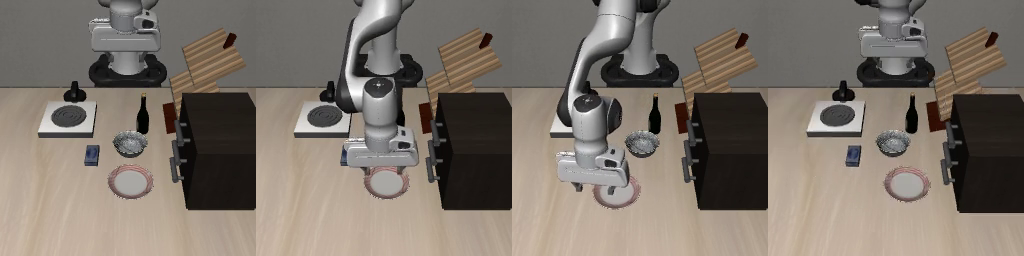
\includegraphics[width=1\linewidth,height=\textheight,keepaspectratio]{../../assets/figures/lecture11/ref/pi0/rollout_keyframes.png}

}

\caption{一次成功 rollout
的四个关键帧，从左到右是同一局内的连续时刻：机械臂从初始位姿探下去、贴住盘沿，再一路把盘子推向炉灶。任务是
libero\_goal
的「把盘子推到炉灶前方」，图片出自本节这段代码------\texttt{code/vla/1\_policy\_rollout/1\_2\_pi0\_libero\_rollout/pi0\_demo.py}（固定初始状态，131
步完成）；第11讲 3.7 节复用的就是这一局}

\end{figure}%

对着这四帧再回看上面那个循环：每一帧画面都是上一个动作造成的后果，也是下一次
\texttt{select\_action} 的输入------第 3
节说的''用自己的动作决定自己下一步看到什么''，在这里是字面意思。四帧之间没有任何人写的分段逻辑：没有''预抓取位姿''、没有状态机、没有阶段校验，全程只有观测进、动作出。这正是第
1 节那条对比的落点。

\subsection{4.4
一个对照实验：把图像换成白噪声}\label{ux4e00ux4e2aux5bf9ux7167ux5b9eux9a8cux628aux56feux50cfux6362ux6210ux767dux566aux58f0}

闭环跑通了，但还剩一个问题没回答：\(\pi_0\)
真的在看图像吗？还是说这个任务本身太固定，光靠本体状态和语言指令就能蒙对？

这个问题不能靠读代码回答，得做对照实验：\textbf{其他一切不动，只把送进网络的图像换成白噪声}，再跑一遍同样的任务，比较两次的成功率。脚本是
\texttt{code/vla/1\_policy\_rollout/1\_2\_pi0\_libero\_rollout/pi0\_test.py}，替换只发生在观测进网络之前的那一步：

\begin{Shaded}
\begin{Highlighting}[]
\KeywordTok{def}\NormalTok{ replace\_images\_with\_white\_noise(observation\_batch: }\BuiltInTok{dict}\NormalTok{[}\BuiltInTok{str}\NormalTok{, Any]) }\OperatorTok{{-}\textgreater{}} \BuiltInTok{dict}\NormalTok{[}\BuiltInTok{str}\NormalTok{, Any]:}
    \ControlFlowTok{for}\NormalTok{ key, value }\KeywordTok{in}\NormalTok{ observation\_batch.items():}
        \ControlFlowTok{if}\NormalTok{ key.startswith(}\StringTok{"observation.images."}\NormalTok{) }\KeywordTok{and}\NormalTok{ torch.is\_tensor(value):}
\NormalTok{            observation\_batch[key] }\OperatorTok{=}\NormalTok{ torch.rand\_like(value)}
    \ControlFlowTok{return}\NormalTok{ observation\_batch}
\end{Highlighting}
\end{Shaded}

注意它只动 \texttt{observation.images.}
开头的键------本体状态、语言指令、动作口径、归一化统计量全都保持原样。这是对照实验的关键：\textbf{一次只改一个变量}，否则成功率掉下来你也说不清是被哪一项改掉的。

把 \texttt{image\_mode} 分别设成 \texttt{"real"} 和
\texttt{"white\_noise"}
各跑一遍，把两次的成功率填进这张表，结论自己就出来了：

\begin{center}
\begin{tabular}{@{}>{\raggedright\arraybackslash}p{\dimexpr 0.1875\linewidth - 2\tabcolsep\relax} >{\raggedright\arraybackslash}p{\dimexpr 0.1562\linewidth - 2\tabcolsep\relax} >{\raggedright\arraybackslash}p{\dimexpr 0.1875\linewidth - 2\tabcolsep\relax}@{}}
\toprule\noalign{}
图像输入 & 其余输入 & 套件成功率 \\
\midrule\noalign{}
真实相机图 & 不变 & ＿＿＿ \\
均匀白噪声 & 不变 & ＿＿＿ \\
\bottomrule\noalign{}
\end{tabular}
\end{center}

怎么读这张表：\textbf{白噪声那一行掉得越多，说明这个策略越依赖视觉。}
如果两行差不多，那就要警惕了------要么这个任务的初始状态太固定、闭着眼睛按固定轨迹走也能成，要么图像那一路根本没接进网络。第二种情况在自己搭推理流水线时并不罕见，而它在成功率上可能一点都不显眼，只有做了这个对照才看得出来。

\subsection{4.5
拿着检查单核对这次部署}\label{ux62ffux7740ux68c0ux67e5ux5355ux6838ux5bf9ux8fd9ux6b21ux90e8ux7f72}

跑通只是第一步。真正把这一讲学透，是拿出 3.5 那张出发前检查单，把这次
\(\pi_0\) + LIBERO 的运行逐行核对一遍：

\begin{itemize}
\tightlist
\item
  \textbf{动作口径}：LIBERO 约定的动作是 7 维的\textbf{相对}增量------前
  3 维是末端位置增量、接着 3 维是姿态（旋转）增量，最后 1
  维控制夹爪开合；环境在内部把增量累加成真实目标，正是 3.3
  说的''相对口径要累加还原''。这份 LIBERO 微调 checkpoint
  就是按这套口径训练的，两端说的是同一种话；一旦把它的输出错当绝对位姿发下去，立刻就是
  3.3
  右图的下场。要提醒的是，这个映射由框架里的输入/输出转换代码（openpi
  那边叫
  \texttt{LiberoInputs}/\texttt{LiberoOutputs}）明确定义，不是权重''自带''的性质------换环境或换框架时，这层转换要重新核对。
\item
  \textbf{归一化统计量}：这份 checkpoint
  把归一化统计量和权重存放在一起，加载策略时一起载入------推理时先把观测归一化送进网络，再把输出反归一化成真实增量。``下载权重就能直接跑''，靠的正是统计量没和权重分家（3.4）。
\item
  \textbf{数值量级}：闭环跑起来之前，可以先打印第一帧的动作看一眼：7
  维增量应当是贴近 0
  的小数。如果看到大数，那是口径或统计量出了问题的信号（3.3、3.4
  的症状），先停下排查，别急着跑完 rollout。
\item
  \textbf{起始位姿}：LIBERO
  每次重置会把机械臂和物体摆到任务定义的初始状态。用\textbf{和微调时一致的环境版本与重置协议}，能显著缩小初始状态的分布差异，3.2
  那个雪球不容易从源头滚起来。但''重置到任务定义的初始分布''不等于''和训练数据分布完全一致''------相机参数、随机化设置、物体姿态、控制器、库版本，以及策略自己走出来的后续状态，都还可能带来偏移。所以仍要用多组初始条件各跑几遍
  rollout，看闭环里有没有漂移。
\item
  \textbf{安全兜底}：仿真里翻车零成本，偶尔的离谱动作顶多让任务失败、摔不坏硬件，这一关可以先放松；但同样的闭环搬上真机之前，裁剪、限速、限位必须补上（3.5）。
\item
  \textbf{评估标准}：判断这次实验成不成，看任务有没有在限定步数内完成，不看
  loss、也不看任何离线数字（3.1、3.2）。
\end{itemize}

检查单六项，每一项都能在这次实验里找到落点。把它核对完，第 3
节那条''训练到部署的来回路''才算真正走通了一遍。

\section{5 本讲小结}\label{ux672cux8bb2ux5c0fux7ed3}

\subsection{5.1
回顾整条数据流}\label{ux56deux987eux6574ux6761ux6570ux636eux6d41}

这一讲只讲了一件事：\textbf{策略，就是从观测到动作的那个网络；用它，就是让''观测→策略→动作→环境→新观测''这个闭环转起来。}
训练时盯成功率而非只盯
loss，部署时把动作口径、归一化统计量、安全边界对齐，这个闭环才转得稳。

\subsection{5.2
策略要吃数据：下一讲采数据}\label{ux7b56ux7565ux8981ux5403ux6570ux636eux4e0bux4e00ux8bb2ux91c7ux6570ux636e}

策略这么强，前提是有数据喂它。\(\pi_0\)
的预训练权重背后，是海量的示教数据。那这些数据从哪来、怎么采、采成什么格式才能直接训练？下一讲就动手采一份能训练的数据集。

\begin{quote}
一句话总结：端到端策略把''感知---规划---控制''的手写流水线，压成一个''观测→动作''的网络；学会它、跑通它的闭环、并在部署时对齐动作口径与归一化，是后面所有
VLA 的起点。
\end{quote}

\section{参考文献}\label{ux53c2ux8003ux6587ux732e}

{[}1{]} CAPUANO F, PASCAL C, ZOUITINE A, et al.~Robot learning: a
tutorial{[}EB/OL{]}. (2025-10-14){[}2026-06-30{]}.
https://arxiv.org/abs/2510.12403.

{[}2{]} BOJARSKI M, DEL TESTA D, DWORAKOWSKI D, et al.~End to end
learning for self-driving cars{[}EB/OL{]}. (2016-04-25){[}2026-06-30{]}.
https://arxiv.org/abs/1604.07316.

{[}3{]} BOJARSKI M, YERES P, CHOROMANSKA A, et al.~Explaining how a deep
neural network trained with end-to-end learning steers a car{[}EB/OL{]}.
(2017-04-25){[}2026-06-30{]}. https://arxiv.org/abs/1704.07911.

{[}4{]} LEVINE S, FINN C, DARRELL T, et al.~End-to-end training of deep
visuomotor policies{[}EB/OL{]}. (2015-04-02){[}2026-06-30{]}.
https://arxiv.org/abs/1504.00702.

{[}5{]} BROHAN A, BROWN N, CARBAJAL J, et al.~RT-1: robotics transformer
for real-world control at scale{[}EB/OL{]}.
(2022-12-13){[}2026-06-30{]}. https://arxiv.org/abs/2212.06817.

{[}6{]} ZHONG Y, BAI F, CAI S, et al.~A survey on vision-language-action
models: an action tokenization perspective{[}EB/OL{]}.
(2025-07-02){[}2026-06-30{]}. https://arxiv.org/abs/2507.01925.

{[}7{]} ROSS S, GORDON G J, BAGNELL J A. A reduction of imitation
learning and structured prediction to no-regret online
learning{[}EB/OL{]}. (2010-11-02){[}2026-06-30{]}.
https://arxiv.org/abs/1011.0686.

{[}8{]} CHI C, XU Z, FENG S, et al.~Diffusion policy: visuomotor policy
learning via action diffusion{[}EB/OL{]}. (2023-03-07){[}2026-06-30{]}.
https://arxiv.org/abs/2303.04137.

{[}9{]} BLACK K, BROWN N, DRIESS D, et al.~\(\pi_0\): a
vision-language-action flow model for general robot control{[}EB/OL{]}.
(2024-10-31){[}2026-06-30{]}. https://arxiv.org/abs/2410.24164.

{[}10{]} LIU B, ZHU Y, GAO C, et al.~LIBERO: benchmarking knowledge
transfer for lifelong robot learning{[}EB/OL{]}.
(2023-06-05){[}2026-06-30{]}. https://arxiv.org/abs/2306.03310.




\end{document}
